\label{chap:sota}

The following chapter reviews the current state of research that motivates an \ac{LLM}-supported workflow for semantic metadata extraction from catalytic experiments.
It first situates this work in \ac{FAIR} catalysis and chemistry data practice, with an emphasis on the difference between making a dataset discoverable and describing its scientific content in a machine-actionable form.
It then introduces application profiles and vocabulary resources that can structure and ground metadata records.
The chapter subsequently discusses domain-aware information extraction, domain-specific language models, and vocabulary grounding as related approaches for turning scientific source material into structured records.
The final section identifies the operational gap that motivates the workflow developed in this thesis.

\section{FAIR Metadata for Catalysis}
\label{sec:fair-data-practice-catalysis}

Catalysis research produces heterogeneous experimental and computational data across publications, instrument exports, local folders, electronic laboratory systems, supplementary files, and repository deposits.
The associated metadata are often fragmented across these environments, which limits machine-readable exchange and later reuse \cite{wulf2021unified,mendes2025data}.
Recent discussions of digital catalysis therefore treat the \ac{FAIR} principles as a response to a practical data problem: available data often lacks the contextual metadata needed for discovery, interpretation, comparison, and later computational use \cite{wilkinson2016fair,marshall2023digital,mendes2021opendata,mendes2025data}.
Related work in chemistry and materials science likewise argues for database-backed and repository-connected infrastructures in which research data are comprehensively described rather than handled only as spreadsheets, local files, or publication supplements \cite{duke2022datastorage,scheffler2022fair}.

Persistent identifiers, repository landing pages, and access protocols address important parts of this problem, but they do not by themselves describe the scientific content of an experiment.
A dataset can be cited, resolved, and indexed while still remaining difficult to search or reuse at the level of catalyst composition, reaction conditions, analytical method, instrument configuration, sample context, or processing history.
Content-level findability and reusability therefore require structured domain metadata in addition to resource-level identifiers.
Repo4Cat and the \ac{NOMAD} catalysis plugin illustrate this direction by combining repository functions with catalysis-specific metadata structures and search capabilities \cite{kushnarenko2025repo4cat,schumann2025nomad}.
Local FAIR infrastructure work similarly connects acquisition, analysis, database upload, relationship generation, and API-based exchange earlier in the laboratory workflow \cite{duke2022datastorage,moshantaf2024advancing}.

For semantic metadata extraction, the important consequence is that \ac{FAIR} practice is not only a publication or repository problem.
It also requires a representation layer that can describe entities, activities, instruments, methods, quantities, units, provenance, and controlled terms in a form that is both machine-actionable and scientifically interpretable.
Application profiles provide this structural layer, while vocabularies and ontologies provide stable identifiers and semantic relations for the concepts used inside it.
The following section therefore focuses on the standards and resources that are most relevant for representing extracted catalysis and chemistry metadata.

\section{Application Profiles and Vocabulary Resources}
\label{sec:semantic-metadata-standards-resources}

Semantic metadata modelling requires both structural specifications and shared semantic resources.
Application profiles define how metadata classes and properties are used in a particular context, including their relations, cardinalities, and value ranges.
Vocabulary resources complement this structure by providing shared identifiers, definitions, synonyms, and semantic relations for domain concepts such as analytical methods, material roles, quantity kinds, units, and spectroscopy-specific parameters \cite{scheffler2022fair,peters2023fair}.
This section first introduces \ac{DCAT-AP+} and \ac{ChemDCAT-AP} as profile resources and then distinguishes the vocabulary resources used for term-level grounding.

\subsection{DCAT-AP+ and ChemDCAT-AP}
\label{sec:dcat-ap-plus-chemdcat-ap}

The design of \ac{DCAT-AP+} is based on a separation between application-profile constraints and ontology semantics.
Its \ac{LinkML} classes and slots define usage-specific node and property shapes, while their \texttt{class\_uri} and \texttt{slot\_uri} mappings refer to classes and properties from external vocabularies.
Consequently, inheritance between LinkML elements specializes their structure and validation constraints but does not itself introduce \ac{OWL} subclass or subproperty axioms.
Multiple shapes can therefore constrain different uses of the same ontology class, while derived domain profiles may retain the generic mappings or replace them with more specific domain terms \cite{dcatapplusDocumentation}.

Within this framework, \ac{DCAT-AP+} defines four design patterns that are central for profile-driven metadata construction, as visualized in \cref{fig:dcat-ap-plus}.
The first pattern is a provenance core that extends the otherwise underspecified use of \ac{PROV-O} in \ac{DCAT-AP}.
A \texttt{dcat:Dataset} is connected through \texttt{prov:wasGeneratedBy} to a \texttt{DataGeneratingActivity}, which is a usage-specific shape mapped to \texttt{prov:Activity}.
The activity can describe used and generated entities, preceding activities, and agentic entities involved in carrying it out.
The more specific \texttt{DataGeneratingActivity} additionally identifies an \texttt{EvaluatedEntity} or \texttt{EvaluatedActivity} representing what was examined during data generation.
Physical instruments and software are represented through \texttt{AgenticEntity} specializations such as \texttt{Device} and \texttt{Software}.
This provenance pattern is important for experimental metadata because it distinguishes the dataset, the activity that generated it, the resources used or produced by that activity, and the scientific object or process being evaluated \cite{dcatapplusDocumentation,stroemert2026chemdcat}.

The provenance pattern also supports data-processing chains.
A \texttt{DataAnalysis} represents an analytical activity, an \texttt{AnalysisSourceData} represents the source data used by that activity, and an \texttt{AnalysisDataset} represents its resulting dataset.
These elements preserve the connection between primary data generation and subsequent analysis without introducing separate ontology classes, because they remain application-profile shapes mapped to \texttt{prov:Activity}, \texttt{prov:Entity}, and \texttt{dcat:Dataset} \cite{dcatapplusDocumentation}.

The second pattern provides generic quantitative and qualitative attributes.
Numerical metadata is represented by \texttt{QuantitativeAttribute}, which is mapped to \texttt{qudt:Quantity} and combines a value with a quantity kind and, where applicable, a unit.
Non-numerical metadata is represented by \texttt{QualitativeAttribute}, which records values such as instrument settings, identifiers, file roles, or categorical observations.
Both attribute types can be attached to entities, activities, devices, or software through generic relations.
They represent recorded metadata values rather than complete ontological models of the underlying physical qualities, which makes them comparatively simple to populate while still preserving the possibility of later specialization by domain profiles \cite{dcatapplusDocumentation}.

The third pattern is flexible classification through the \texttt{ClassifierMixin}, which adds both \texttt{rdf\_type} and \texttt{type} to central \ac{DCAT-AP+} shapes.
The \texttt{rdf\_type} slot maps to \texttt{rdf:type} and expresses that an instance belongs to a class from a formal ontology.
In contrast, \texttt{type} maps to \texttt{dcterms:type} and provides lightweight categorization using a controlled-vocabulary term, such as a \ac{SKOS} concept, without asserting formal class membership.
This distinction allows domain-specific semantics to be added to individual instances without requiring a separate \ac{OWL} subclass for every type of activity, entity, instrument, or attribute \cite{dcatapplusDocumentation}.

The fourth pattern provides optional contextual metadata through the \texttt{Plan} and \texttt{Surrounding} shapes.
A \texttt{Plan}, mapped to \texttt{prov:Plan}, represents directive information such as a method, protocol, or standard operating procedure and is linked to a \texttt{DataGeneratingActivity} through \texttt{realized\_plan}.
A \texttt{Surrounding}, mapped to \texttt{prov:Location}, represents the spatial context in which data generation occurred, such as a laboratory, field site, or computational environment, and is linked through \texttt{occurred\_in}.
These shapes are intentionally minimal and can be classified or extended by domain profiles \cite{dcatapplusDocumentation}.

\begin{figure}[H]
    \centering
    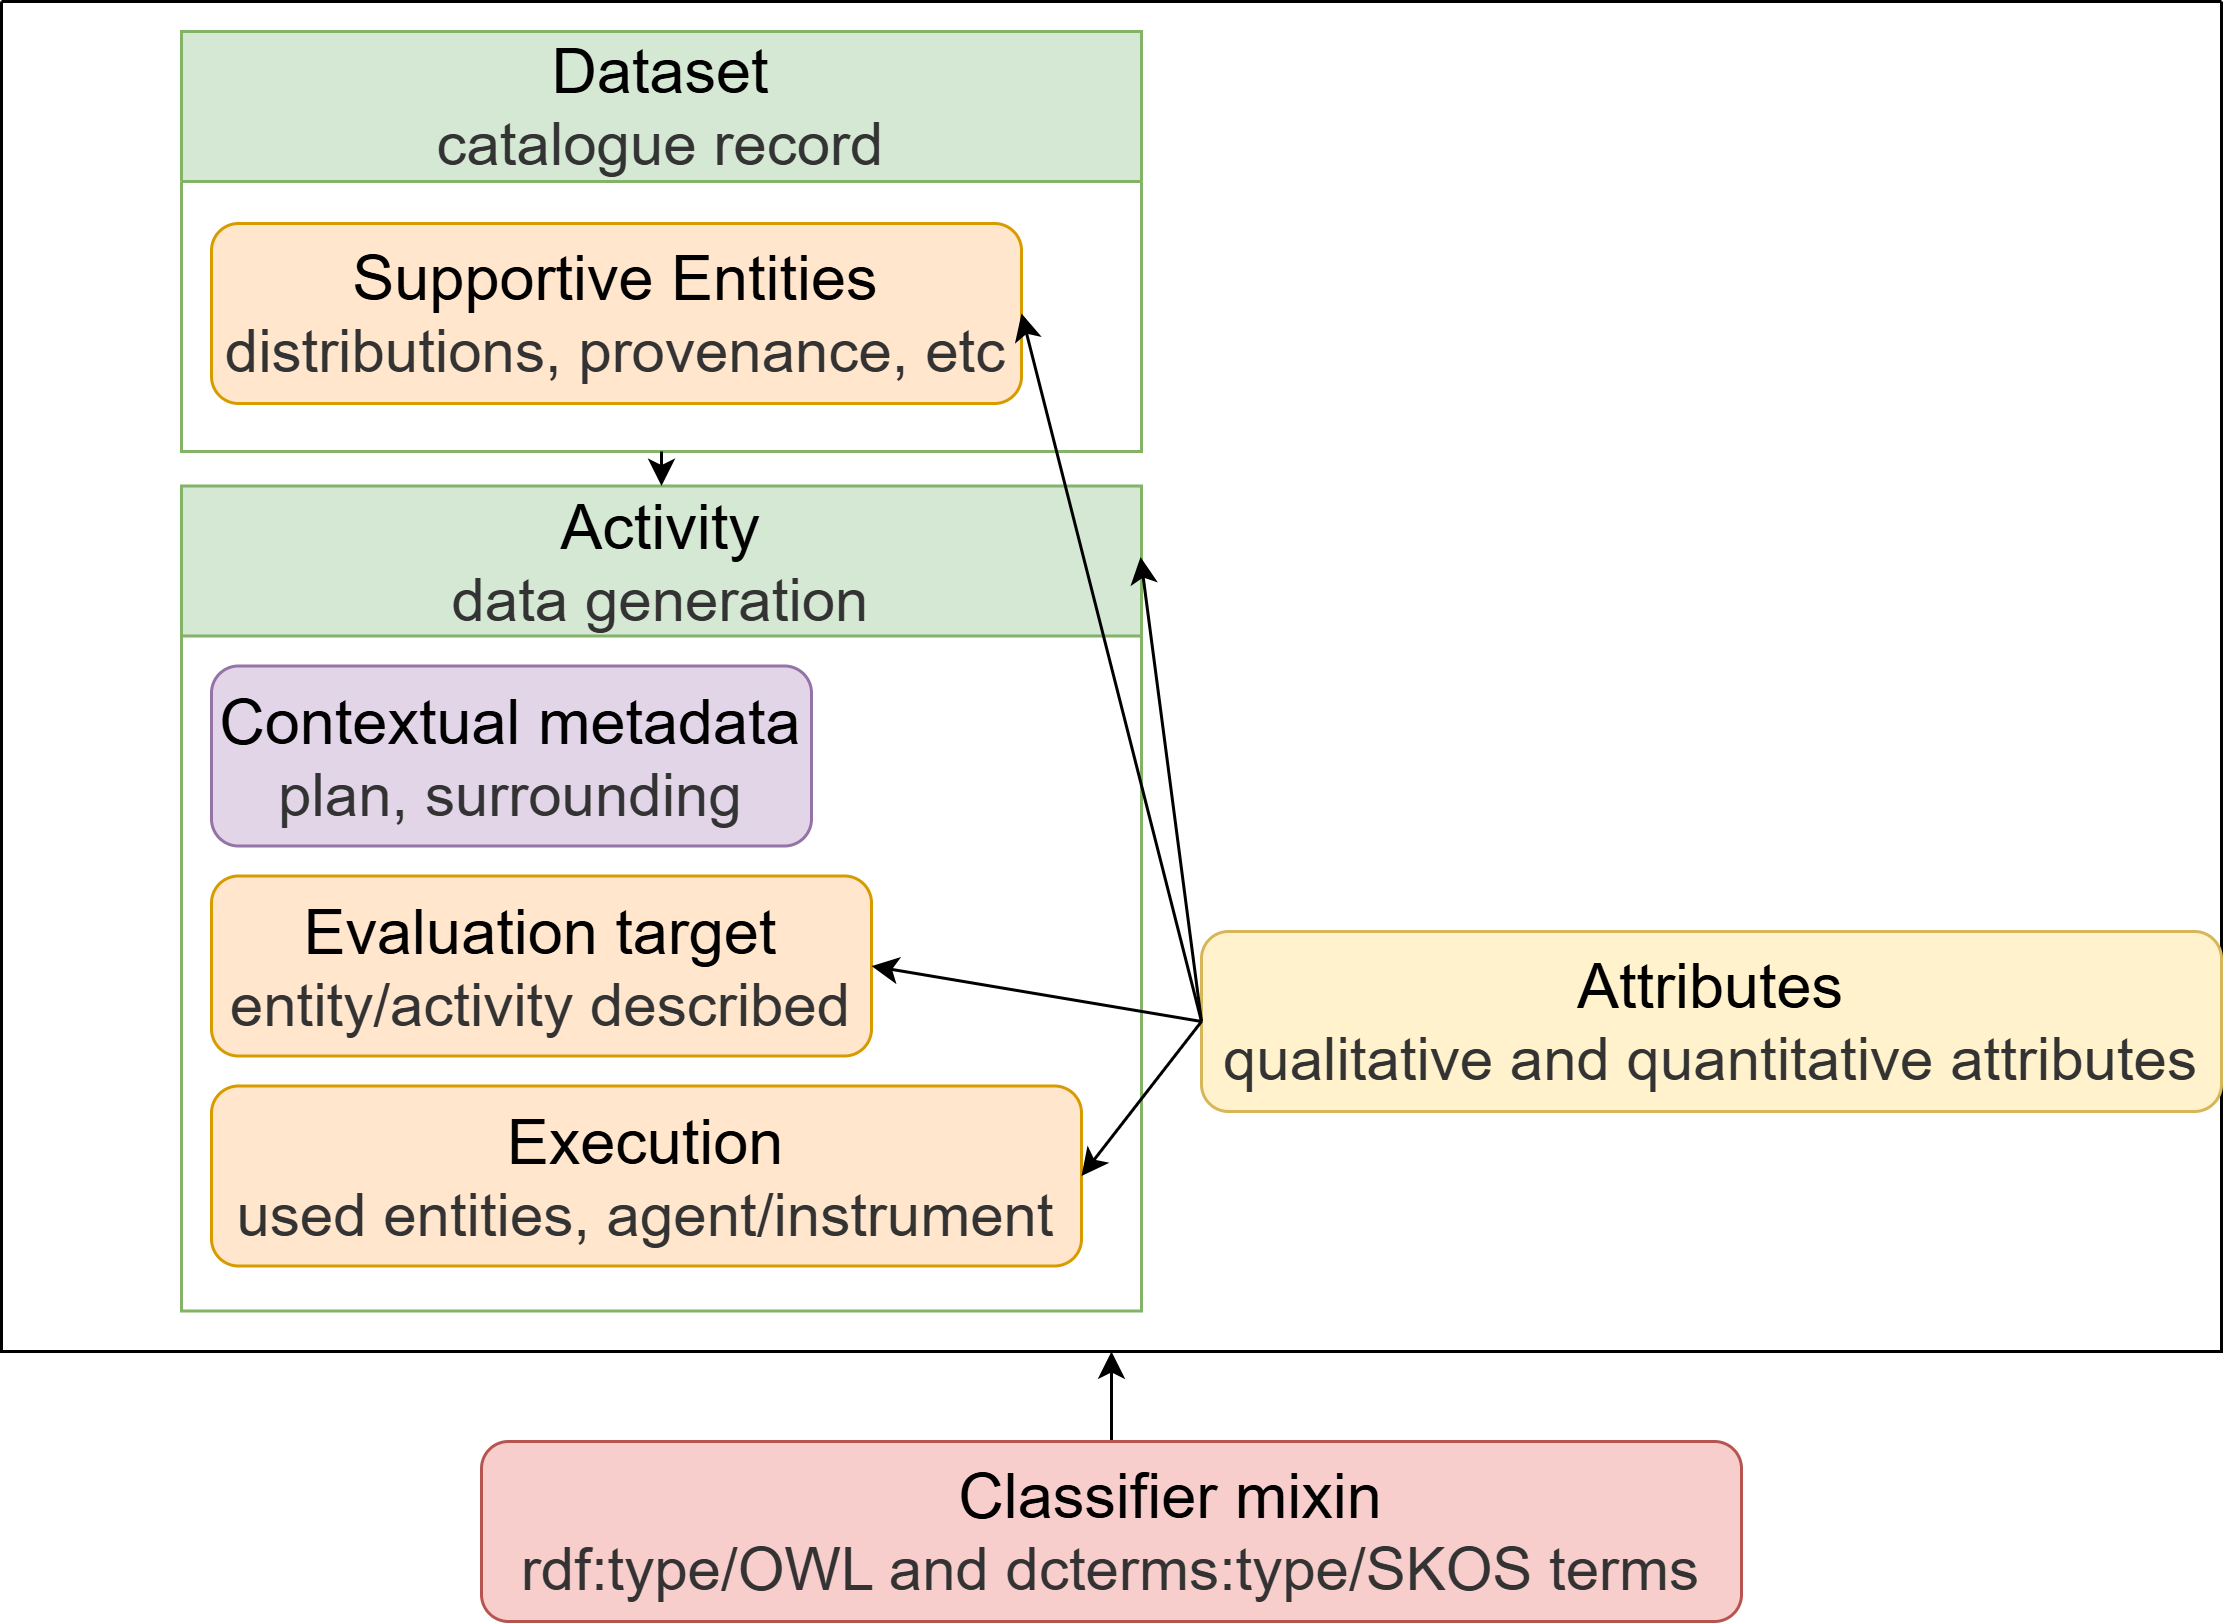
\includegraphics[width=0.74\textwidth]{figures/dcat_ap_plus.png}
    \caption{Central \ac{DCAT-AP+} profile patterns used for provenance-oriented dataset description, generic quantitative and qualitative attributes, controlled classification, and optional contextual metadata.}
    \label{fig:dcat-ap-plus}
\end{figure}

\ac{ChemDCAT-AP} is the first domain-specific application profile built on \ac{DCAT-AP+} and provides a shared metadata foundation for chemistry- and catalysis-related research data \cite{stroemert2026chemdcat,chemdcatapDocumentation}.
It imports the generic provenance, attribute, classification, and contextual patterns of \ac{DCAT-AP+} and specializes them through \ac{LinkML} inheritance.
ChemDCAT-AP classes extend corresponding \ac{DCAT-AP+} shapes through \texttt{is\_a}, while domain-specific slots specialize generic relations in the same manner.
Their mappings refer to established semantic resources including ChEBI, CHEMINF, the Semanticscience Integrated Ontology, and the Named Reaction Ontology.
This preserves structural compatibility with the generic profile while producing more precise \ac{RDF} and narrower validation constraints for chemical metadata \cite{stroemert2026chemdcat,chemdcatapDocumentation}.

The profile is organized into modules for material entities, chemical entities, chemical reactions, and their integration with the dataset and data-generation patterns inherited from \ac{DCAT-AP+}.
Material samples and substance samples are modeled as entity specializations, while chemical reactions are modeled as activity specializations.
Roles involved in a reaction are represented through shapes such as \texttt{StartingMaterial}, \texttt{Reagent}, \texttt{ChemicalProduct}, \texttt{Catalyst}, and \texttt{Reactor}.
ChemDCAT-AP also specializes generic attribute and provenance relations.
Instead of representing recurring chemical identifiers or quantities only through generic attributes and instance-level classifications, dedicated slots such as \texttt{inchi}, \texttt{inchikey}, \texttt{smiles}, \texttt{has\_temperature}, \texttt{has\_mass}, and \texttt{has\_yield} encode common chemical meanings directly in the schema \cite{stroemert2026chemdcat,chemdcatapDocumentation}.

ChemDCAT-AP remains a foundational rather than exhaustive reporting profile.
Its generic chemical dataset and activity shapes are intended to be further constrained by use-case-specific profiles that define required properties, cardinalities, and controlled terms for particular methods or subdomains.
This extension mechanism is important for analytical and catalysis metadata because a generic chemistry profile can provide reusable provenance and attribute patterns, while method-specific profiles can decide which acquisition settings, sample descriptors, instrument parameters, or processing details are required for a curator-facing record \cite{stroemert2026chemdcat,chemdcatapDocumentation}.

\subsection{Vocabulary Resources}
\label{sec:vocabulary-resources}

Application profiles and vocabularies contribute different parts of semantic metadata modelling.
The profile defines the structure of a record, while vocabulary resources provide stable identifiers for the terms used inside that structure.
For metadata extraction, this distinction matters because a workflow may identify a value, place it in a profile field, and only then map its label or unit to a controlled term.
The following resources illustrate three different scopes of grounding: broad catalysis terminology, cross-domain quantity semantics, and NMR-specific spectroscopy metadata.

\subsubsection{Voc4Cat}
\label{sec:voc4cat}

\ac{Voc4Cat} is a community-maintained \ac{SKOS} vocabulary developed within \ac{NFDI4Cat} for catalysis-related disciplines.
It assigns stable, resolvable \acp{URI} to catalysis concepts and provides preferred labels, alternative labels, definitions, and hierarchical relations \cite{david_linke_2023_8313340,nfdi4cat2024whitepaper}.
As a \ac{SKOS} resource, Voc4Cat is suited to lightweight classification, indexing, terminology-based retrieval, and vocabulary alignment.
A metadata record can reference a Voc4Cat concept as the value of a classification or annotation property without thereby asserting that the described resource is an instance of a corresponding \ac{OWL} class \cite{w3c2009skos}.

For example, Voc4Cat identifies \enquote{nuclear magnetic resonance spectroscopy} through a catalysis-relevant characterization concept.
This can normalize lexical variants such as \texttt{NMR} and \texttt{nuclear magnetic resonance spectroscopy} at the method level.
However, broader catalysis terminology does not replace a method-specific resource when the metadata model needs to preserve more specific details such as observed nucleus, pulse sequence, raw signal type, or processing state.

\subsubsection{Quantities, Units, Dimensions and Types Ontology (QUDT)}
\label{sec:qudt}

The \acf{QUDT} provides a cross-domain semantic model for quantities, quantity kinds, units of measure, dimensions, numerical values, and their machine-readable representations.
It complements domain vocabularies such as Voc4Cat by providing identifiers and relations needed to express the quantitative semantics of measurements and attributes.
A literal value such as \texttt{400} becomes explicit and machine-actionable when it is linked, for example, to \texttt{quantitykind:\allowbreak Frequency} and \texttt{unit:\allowbreak MegaHZ} \cite{qudt2022schema}.

QUDT also provides relations for unit--quantity-kind compatibility.
The quantity-kind resource \texttt{quantitykind:\allowbreak Frequency} is linked to compatible unit resources such as \texttt{unit:\allowbreak HZ} and \texttt{unit:\allowbreak MegaHZ}, while the corresponding unit resources are associated with quantity kinds through \texttt{qudt:\allowbreak hasQuantityKind} \cite{qudt2022schema}.
These relations can support validation and transformation software, for example by checking whether a frequency value is paired with a frequency unit or by converting a value to a selected reference unit.
At the same time, QUDT is not a domain vocabulary for spectroscopy or catalysis; it can represent quantitative compatibility, but it does not by itself decide which scientific object a value describes.

\subsubsection{NMR Controlled Vocabulary (nmrCV)}
\label{sec:nmr-cv}

The \ac{nmrCV} is the controlled vocabulary accompanying \ac{nmrML}, an open, vendor-neutral \ac{XML} format for exchanging and storing \ac{NMR} data.
While the \ac{nmrML} schema defines the document structure, nmrCV supplies standardized identifiers for spectroscopy-specific concepts concerning instrumentation, acquisition, spectral data processing, and spectral interpretation \cite{Schober2018nmrML}.
Together, nmrML and nmrCV express a view of NMR metadata in which reusable data requires more than a plotted spectrum: raw free-induction decay data, acquisition settings, instrument configuration, sample and reference context, processing metadata, assignments, and chemical-structure information may all be needed to preserve the meaning of an experiment \cite{Schober2018nmrML}.

The scope of nmrCV therefore complements broader resources such as Voc4Cat and QUDT.
It can identify spectroscopy-specific concepts such as instrument and acquisition parameters, raw or processed data products, and processing operations.
Examples include terms for an NMR probe, pulse-related acquisition settings, \ac{FID} data, peak-picked spectra, and baseline correction \cite{Schober2018nmrML}.
This makes nmrCV relevant when a metadata record must distinguish a generic NMR characterization method from the more specific acquisition and processing facts that make an NMR dataset interpretable.

\section{Domain-Aware Information Extraction}
\label{sec:domain-aware-information-extraction}

The application profiles and vocabularies discussed above define how catalysis and chemistry metadata can be represented, but much of the information required to populate these structures is available only in unstructured or semi-structured form.
Scientific publications distribute relevant information across prose, tables, captions, and figures, while experimental data packages may include supplementary files, reports, instrument exports, spreadsheets, images, and locally maintained metadata files \cite{schilling2025text,Fan2024OpenChemIE}.
Constructing semantic metadata is therefore not only a modelling task, but also an acquisition and information-integration task.

ChemDataExtractor is a foundational example of chemistry-aware information extraction.
It combines chemical named-entity recognition, rule-based parsing grammars, and document-level processing to extract chemical entities together with associated properties, measurements, and relations from scientific documents \cite{swain2016chemdataextractor}.
Its relevance for metadata extraction lies in the explicit treatment of chemistry as a domain with specialized entities, not as generic prose.
Zhang et al.\ extend this domain-aware perspective into catalysis by constructing a full-text catalysis information-extraction benchmark and an extraction pipeline for six entity types: catalyst, reaction, reactant, product, characterization, and treatment \cite{zhang2022knowledge}.
Their workflow combines article selection, active-learning-assisted annotation, span-based entity extraction, and entity normalization, and uses extracted entities in an entity-aware search engine and a co-occurrence-based correlation analysis system.
This work is important for catalysis-related metadata extraction because it shows the value of explicit domain categories and annotated extraction targets, while remaining closer to entity extraction and search than to profile-level semantic metadata construction.

Generative \ac{LLM} workflows extend information extraction from predefined labels toward structured records governed by a user-specified target representation.
CatMiner applies this pattern to heterogeneous catalysis literature by extracting user-specified structure--environment--property records through sequential prompting, domain-specific instructions, follow-up checks, and searches for relevant context across sentences and paragraphs \cite{walls2025catminer}.
Its evaluation against a handmade database, together with manual verification of selected extracted records, illustrates that even domain-specific \ac{LLM} extraction remains tied to ground-truth construction, validation, and review.
The reported error cases, including vague catalyst names, unrelated context, and confusion between different temperature roles, also show that domain-specific extraction requires more than syntactically valid output \cite{walls2025catminer}.

SPIRES provides a complementary schema-guided approach.
It recursively interrogates an \ac{LLM} according to a user-defined nested schema and grounds extracted entities against external ontologies and controlled vocabularies \cite{caufield2024spires}.
The method is designed to assist manual knowledge curation and acquisition while using public databases and ontologies for validation.
This is relevant for semantic metadata extraction because it separates the target schema, the extraction prompts, and the grounding step, rather than relying on an unconstrained text summary.
At the same time, SPIRES discusses hallucination and relation-extraction errors as remaining reliability concerns, which keeps human validation within the workflow rather than outside it \cite{caufield2024spires}.

EDC addresses knowledge-graph construction from text through three phases: open information extraction, schema definition, and post-extraction canonicalization \cite{zhang2024edc}.
It can operate with either a predefined target schema or a schema induced from extracted information, and it retrieves relevant schema elements when the complete schema is too large for the prompt.
This provides a different design precedent from fixed-label extraction: source signals may first be collected more openly, then organized and canonicalized against a schema.
Together, CatMiner, SPIRES, and EDC illustrate several ways of combining domain knowledge, schemas, evidence selection, and canonical identifiers during \ac{LLM}-based extraction.

Domain-aware extraction also depends on the semantic model used to interpret extracted roles.
Reac4Cat-Ontology is not primarily an extraction pipeline, but it demonstrates why catalysis roles and relations often require explicit semantic modelling.
It uses \ac{OWL} description logic and general class axioms to infer reaction roles, catalyst participation, and reaction classifications from formally represented component relations \cite{behr2024reac4cat}.
For metadata extraction, this reinforces the distinction between detecting a domain term and assigning it to the correct role in a structured record.
A catalyst, reagent, product, analytical method, or acquisition parameter is not only a label; it receives its meaning from the entity, activity, relation, and context in which it is placed.

\section{Domain-Specific Models, Retrieval, and Grounding}
\label{sec:domain-specific-models-retrieval-grounding}

The extraction workflows above also depend on how well the underlying language representations capture scientific and domain-specific terminology.
SciBERT shows that pretraining on scientific text improves performance on scientific sequence tagging, sentence classification, and parsing tasks compared with general-domain representations \cite{beltagy2019scibert}.
MatSciBERT narrows this idea further by pretraining on materials-science literature and reporting improvements for named-entity recognition, relation classification, and abstract classification in materials-domain tasks \cite{gupta2022matscibert}.
In chemistry, Zhang et al.\ evaluate fine-tuned \acp{LLM} on chemical text-mining tasks including compound entity recognition, reaction role labelling, MOF synthesis extraction, NMR data extraction, and reaction paragraph-to-action-sequence conversion \cite{zhang2024chemicaltextmining}.
These studies support the general observation that scientific terminology, formulas, abbreviations, and role distinctions can require domain-adapted representations or task-specific tuning.

For semantic metadata extraction, this observation applies not only to generation but also to retrieval and grounding.
Vocabulary grounding depends on query formulation, lexical and embedding-based candidate retrieval, and selection among nearby but semantically different terms.
Domain-specific language models or rerankers can therefore be relevant when source expressions, profile fields, and vocabulary labels differ in wording but refer to related concepts.
However, grounding and retrieval solve a different problem from profile construction.
They can normalize or disambiguate terms that have already been exposed as candidate values, but they do not by themselves decide which entity or activity should own a value, whether a quantity describes an instrument, a sample, or a processing step, or whether a source fact should become metadata at all.

The literature therefore points to a layered distinction between evidence detection, schema-oriented organization, and term-level grounding.
ChemDataExtractor and catalysis IE work emphasize domain-aware entities and annotated extraction targets \cite{swain2016chemdataextractor,zhang2022knowledge}.
CatMiner, SPIRES, and EDC show different ways of combining schemas, domain instructions, context search, ontology grounding, and canonicalization in \ac{LLM}-based extraction workflows \cite{walls2025catminer,caufield2024spires,zhang2024edc}.
Domain-specific encoders and fine-tuned models provide evidence that scientific text processing can benefit from representations adapted to the language of the field \cite{beltagy2019scibert,gupta2022matscibert,zhang2024chemicaltextmining}.
The open question for a metadata workflow is how these layers behave when they are combined for heterogeneous experimental packages rather than only for article-centered extraction tasks.

\section{Research Gap}
\label{sec:research-gap}

The literature reviewed in this chapter shows that the central gap is not a lack of individual building blocks.
Catalysis and chemistry research already provide \ac{FAIR} infrastructure initiatives, repository concepts, semantic metadata profiles, controlled vocabularies, NMR metadata resources, catalysis-specific extraction benchmarks, chemistry-aware information extraction systems, schema-guided \ac{LLM} extraction approaches, and ontology-grounding methods \cite{nfdi4cat2024whitepaper,steinbeck2023nfdi4chem,kushnarenko2025repo4cat,schumann2025nomad,stroemert2026chemdcat,david_linke_2023_8313340,Schober2018nmrML,swain2016chemdataextractor,zhang2022knowledge,walls2025catminer,caufield2024spires,zhang2024edc}.
Taken together, these works provide strong building blocks for semantic metadata extraction.
Comparatively less developed, however, is evidence on how these building blocks behave when combined into an inspectable end-to-end workflow for heterogeneous experimental dataset packages.

Existing extraction systems are strongest where the input is a scientific article, a controlled text corpus, or a schema-guided extraction task over selected passages.
Experimental data packages can instead contain PDFs, spreadsheets, local metadata files, images, instrument exports, supplementary tables, binary resources, and partially structured folders.
The information needed for a metadata profile may therefore be distributed across document types and may not follow the rhetorical structure of a journal article.
This creates an operational challenge: the workflow must preserve source evidence, distinguish file-level orientation from evidence, identify domain-relevant signals, construct a profile-shaped metadata draft, ground selected fields against controlled resources, and keep the resulting artifacts inspectable.

A second gap concerns the relation between schema validity, semantic adequacy, and curation.
Schema-valid output is necessary for machine-actionable metadata, but it does not by itself prove scientific correctness.
A generated record can satisfy a profile schema while still assigning a value to the wrong entity, losing unit context, omitting an acquisition fact, or grounding a term to an inappropriate vocabulary concept.
The reviewed literature therefore supports the need to treat evidence, profile structure, vocabulary grounding, validation, and human review as complementary controls rather than interchangeable guarantees \cite{schilling2025text,walls2025catminer,caufield2024spires}.

This thesis is positioned in that operational integration gap.
It does not propose a new catalysis ontology, a new repository, or a fully automated literature database.
Instead, the workflow developed in this thesis investigates how heterogeneous source handling, evidence-oriented extraction, metadata profile projection, semantic review, vocabulary grounding, validation, and artifact-based diagnosis can be connected in one prototype workflow.
The contribution is therefore not the replacement of existing standards, vocabularies, or extraction systems, but an examination of how they can be made usable as constraints and grounding resources in an \ac{LLM}-supported metadata extraction process.
